\documentclass[crop=false,fleqn]{standalone}
\usepackage{../../../globle-preamble}

\begin{document}
    \textbf{Find the domain and range of the funtion $g$ and sketch graph of $g$.}

    $$ g(x) = \sqrt{x^2-4} $$

    \vspace{1em}
    Domain of $g(x)$ = $\mathbb{R} - (-2, 2)$

    Range of $g(x)$ = $[0,+\infty)$
    \vspace{1em}

    \begin{center}
        \begin{tabular}{ |c|c|c|c|c|c|c| } 
            \hline
            $x$ & -4 & -3 & -2 & 2 & 3 & 4 \\ 
            \hline
            $g(x)$ & $2\sqrt{3}$ & $\sqrt{5}$ & 0 & 0 & $\sqrt{5}$ & $2\sqrt{3}$ \\
            \hline
        \end{tabular}
    \end{center}

    \begin{center}
        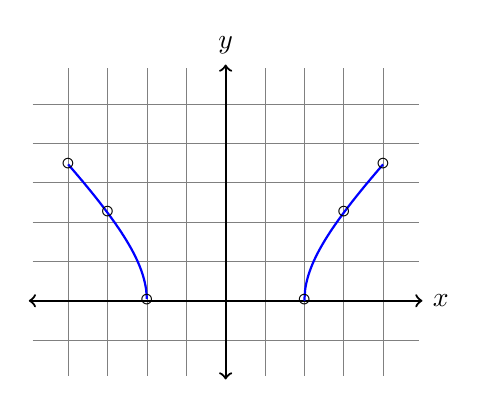
\begin{tikzpicture}[scale=0.5]
            \draw[step=1,gray,very thin] (-4.9,-1.9) grid (4.9,5.9);
            \draw[<->,thick] (-5, 0) -- (5, 0) node[right] {$x$};
            \draw[<->,thick] (0, -2) -- (0, 6) node[above] {$y$};
            
            \draw[domain=-4:-2, samples=105, smooth, variable=\x, thick, blue]
                plot ({\x}, {sqrt(\x*\x-4)});
            \draw[domain=2:4, smooth, variable=\x, thick, blue, samples=100]
                plot ({\x}, {sqrt(\x*\x-4)});

            \foreach \Point in {(-4,3.4641), (-3,2.236), (-2,0), (2,0), (3,2.236), (4,3.4641)}{
                \node at \Point {$\circ$};
            }
        \end{tikzpicture}
    \end{center}
\end{document}
